\chapter{METODOLOGI}
\label{chap:metodologi}

% Ubah bagian-bagian berikut dengan isi dari desain dan implementasi

Penelitian ini dilaksanakan sesuai dengan metodologi yang tertera pada bab ini. Metodologi yang digunakan dalam penelitian ini adalah sebagai berikut:

\section{Data dan Peralatan}
Adapun tata pendukung berupa data dan peralatan yang digunakan dalam pelaksanaan penelitian tugas akhir ini adalah sebagai berikut:

\subsection{Data}

Data yang akan digunakan dalam penelitian ini adalah data citra yang diperoleh dari hasil pengambilan gambar secara manual menggunakan kamera di gerbang tol. Data citra tersebut akan digunakan sebagai data latih dan data uji dalam proses pelatihan model dan pengujian model. Data citra tersebut akan diolah dan diolah menggunakan teknik visi komputer untuk mendeteksi apakah kendaraan yang melintas adalah kendaraan yang \emph{overdimension} atau tidak.

\subsection{Peralatan}

Adapun peralatan yang digunakan dalam penelitian tugas akhir ini adalah sebagai berikut:

\begin{itemize}[noitemsep,nolistsep]
  \setlength{\itemsep}{7pt}
  \setlength{\parskip}{0pt}
  \setlength{\parsep}{0pt}
  \item Visual Studio Code
  \item Jetson Nano Developer Kit
  \item Beelink Gemini T34
  \item Tripod
  \item Webcam
  \item \emph{Server Cloud}
  \item \emph{Smartphone Android}
  \item Laptop
\end{itemize}

Tugas akhir ini akan dilaksanakan sesuai dengan desain sistem beserta implementasinya yang akan dibahas pada bab ini. Desain sistem ini merupakan konsep dasar perancangan dan pembuatan program pada tugas akhir ini. Desain sistem ini direpresentasikan dalam bentuk blok diagram yang diselesaikan secara bertahap dan menyeluruh.

\section{Metode yang Digunakan}

Adapun tugas akhir ini merupakan pengembangan dari teknologi visi komputer yang kemudian diimplementasikan pada \emph{Jetson Nano Developer Kit} dan \emph{Beelink Gemini T34}. Secara umum, pelaksanaan tugas akhir ini didasari oleh blok diagram yang dapat dilihat pada \textbf{Gambar \ref{fig:blockdiagrammethod}}.

\begin{figure}[H]
  \centering

  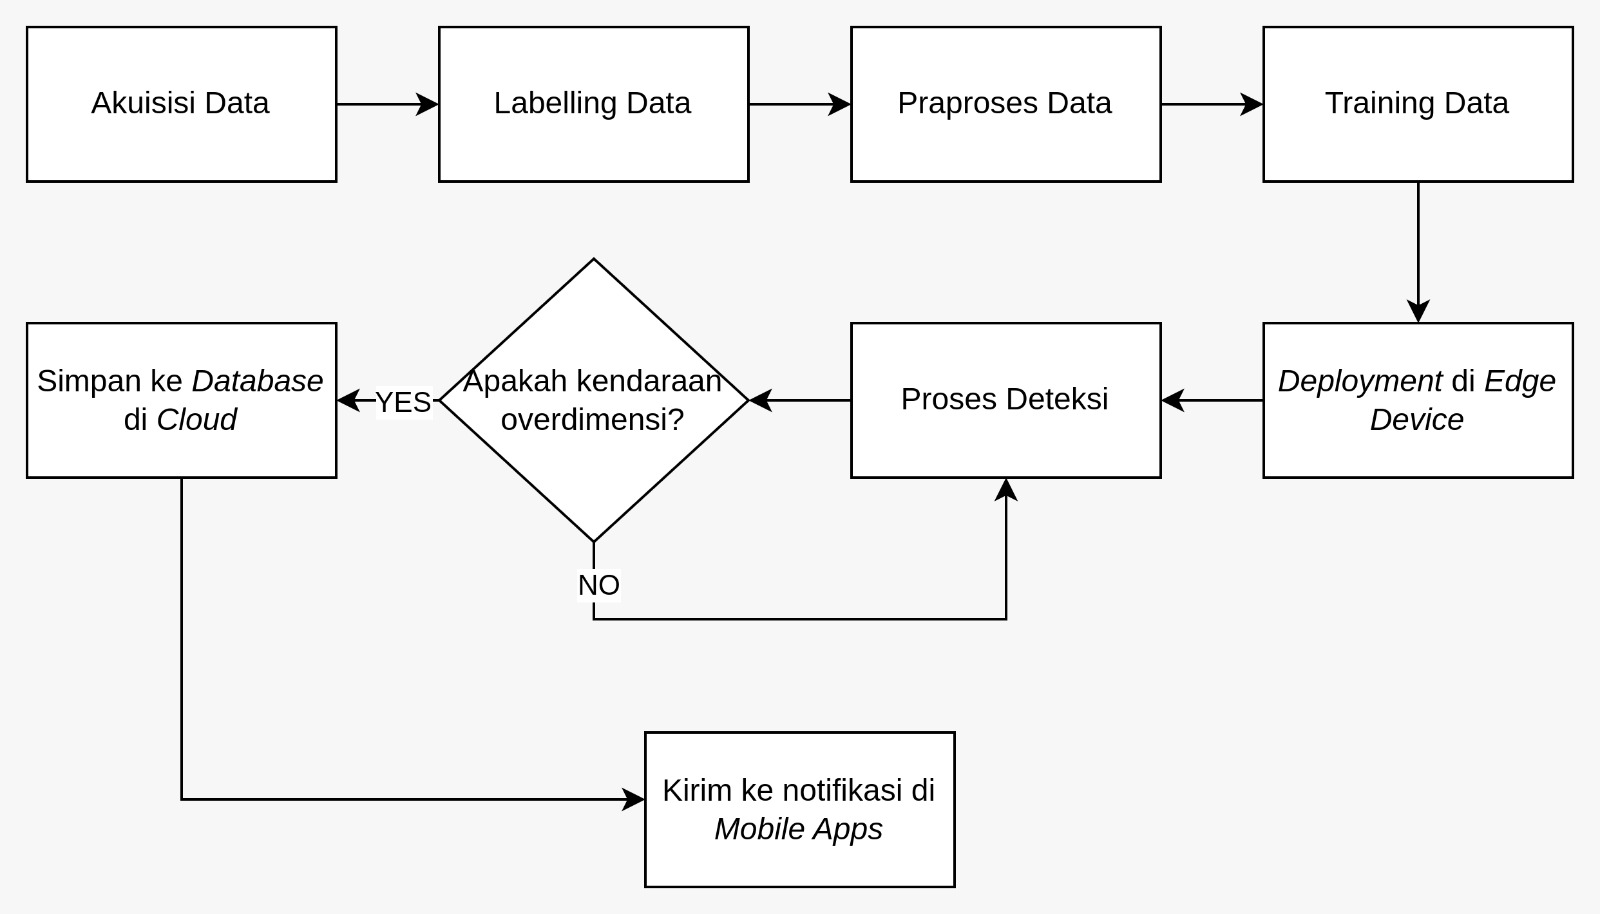
\includegraphics[scale=0.25]{gambar/bab3-block-diagram.jpeg}

  \caption{Blok diagram metodologi}
  \label{fig:blockdiagrammethod}
\end{figure}

\subsection{Akuisisi Data}

Pada tahap ini, data citra yang diperoleh dari hasil pengambilan gambar secara manual menggunakan kamera di gerbang tol. Data citra tersebut akan digunakan sebagai data latih dan data uji dalam proses pelatihan model dan pengujian model. Data citra tersebut akan diolah dan diolah menggunakan teknik visi komputer untuk mendeteksi apakah kendaraan yang melintas adalah kendaraan yang \emph{overdimension} atau tidak.

\subsection{Labelling Data}

Pada tahap ini, data citra yang telah diperoleh akan dilakukan labelling. Labelling data dilakukan dengan cara memberikan label pada data citra yang telah diperoleh. Label yang diberikan adalah label yang menunjukkan apakah kendaraan yang melintas adalah kendaraan yang \emph{overdimension} atau tidak.

\subsection{Praproses Data}

Pada tahap ini, data citra yang telah dilabeli akan dilakukan praproses. Praproses data dilakukan dengan cara melakukan augmentasi data. Augmentasi data dilakukan dengan cara melakukan rotasi, pergeseran, dan perubahan warna pada data citra. Hal ini dilakukan untuk memperbanyak variasi data citra yang akan digunakan dalam proses pelatihan model.

\subsection{Training Data}

Pada tahap ini, data citra yang telah dilabeli dan dipreproses akan dilakukan pelatihan model. Pelatihan model dilakukan dengan cara membagi data citra menjadi dua bagian, yaitu data latih dan data validasi. Data latih digunakan untuk melatih model sedangkan data validasi digunakan untuk menguji model. Model yang digunakan adalah model \emph{SSD MobileNetV2}.

\subsection{Deployment di \emph{Edge Device}}

Pada tahap ini, model yang telah dilatih akan diimplementasikan pada \emph{Jetson Nano Developer Kit} dan \emph{Beelink Gemini T34}. Implementasi model dilakukan dengan cara mengubah model yang telah dilatih menjadi model yang dapat dijalankan pada \emph{Jetson Nano Developer Kit} dan \emph{Beelink Gemini T34}. Model yang diimplementasikan adalah model \emph{SSD MobileNetv2}.

\subsection{Proses Deteksi}

Pada tahap ini, model yang telah diimplementasikan akan digunakan untuk mendeteksi apakah kendaraan yang melintas adalah kendaraan yang \emph{overdimension} atau tidak. Proses deteksi dilakukan dengan \emph{live inferencing} pada \emph{Jetson Nano Developer Kit} dan \emph{Beelink Gemini T34}. Hasil deteksi akan ditampilkan pada layar monitor.

\subsection{Penyimpanan Data ke \emph{Cloud}}

Pada tahap ini, hasil deteksi yang telah dilakukan akan disimpan ke server cloud. Proses penyimpanan data dilakukan dengan cara mengirimkan data hasil deteksi ke database cloud. Data hasil deteksi yang disimpan yaitu:

\begin{itemize}[noitemsep,nolistsep]
  \setlength{\itemsep}{5pt}
  \setlength{\parskip}{0pt}
  \setlength{\parsep}{0pt}
  \item ID
  \item Jenis kendaraan
  \item Waktu deteksi
  \item Overdimension atau tidak
  \item Gambar kendaraan
\end{itemize}

Diagram basis data yang digunakan dapat dilihat pada \textbf{Gambar \ref{fig:dbdiagram}}.

\begin{figure}[H]
  \centering

  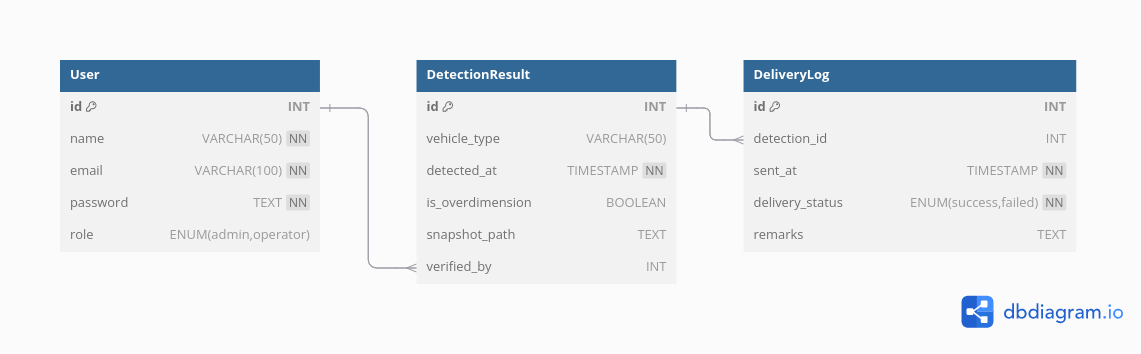
\includegraphics[scale=0.39]{gambar/bab3-basis-data.png}

  \caption{Diagram basis data}
  \label{fig:dbdiagram}
\end{figure}

Struktur basis data yang digunakan terdiri dari tiga tabel utama, yaitu:

\begin{enumerate}[nolistsep,label=\textbf{\arabic*.}]

  \item \textbf{Tabel User}: Tabel ini digunakan untuk menyimpan informasi pengguna sistem, seperti nama, email, kata sandi, dan peran pengguna (administrator atau operator). Struktur ini memungkinkan sistem untuk mengatur akses berdasarkan peran pengguna, sehingga keamanan dan tanggung jawab penggunaan sistem dapat terjaga.
  \item \textbf{Tabel DetectionResult}: Tabel ini merupakan inti dari sistem, yang menyimpan informasi hasil deteksi kendaraan. Data yang dicatat meliputi jenis kendaraan, waktu deteksi, status overdimensi, serta jalur penyimpanan gambar kendaraan. Selain itu, tabel ini juga memiliki kolom untuk mencatat identitas pengguna yang memverifikasi hasil deteksi.
  \item \textbf{Tabel DeliveryLog}: Tabel ini berfungsi mencatat log pengiriman data hasil deteksi ke cloud. Informasi yang disimpan meliputi waktu pengiriman, status pengiriman (berhasil atau gagal), dan keterangan tambahan, seperti pesan kesalahan jika pengiriman mengalami kegagalan. Tabel ini penting untuk melacak riwayat pengiriman dan mendukung analisis jika terjadi kendala teknis.
\end{enumerate}

\subsection{Pengiriman Notifikasi ke \emph{Mobile Apps}}

Pada tahap ini, hasil deteksi yang telah disimpan ke server cloud akan dikirimkan notifikasi ke aplikasi \emph{mobile}. Proses pengiriman notifikasi dilakukan dengan cara mengirimkan notifikasi ke aplikasi \emph{mobile} yang terhubung dengan \emph{server cloud}. Notifikasi yang dikirimkan berupa notifikasi apakah kendaraan yang melintas adalah kendaraan yang \emph{overdimension} atau tidak.